\documentclass[letterpaper,conference]{IEEEtran}

\usepackage{cite}
\usepackage{amsmath,amssymb}
\usepackage{newtxtext,newtxmath}
\usepackage{graphicx}
\usepackage{booktabs}
\usepackage{url}
\usepackage{xcolor}
\usepackage{tikz}
\usetikzlibrary{arrows.meta,positioning,fit}

\definecolor{stageblue}{RGB}{34,91,142}
\definecolor{stagefill}{RGB}{235,242,248}
\definecolor{reviewfill}{RGB}{255,246,215}
\definecolor{rejectfill}{RGB}{252,232,232}

\begin{document}

\title{Evidence-Bound Reconstruction of Planar Unity Worlds from Stationary Nadir Drone Video}

\author{\IEEEauthorblockN{Harsh Ranjan, Devroop Dasgupta, Deepak Baghel, and Aman Dev}
\IEEEauthorblockA{Mentor: Dr. Savitha Choudhary}}

\maketitle

\begin{abstract}
Converting a short aerial video into an editable game-engine scene requires a static surface, spatial calibration, actor trajectories, semantic structure, and an explicit account of what the camera cannot measure. This paper presents an evidence-bound pipeline for cut-free, stationary, approximately nadir video of a planar scene. It audits consecutive frames, compensates bounded hover and smooth zoom, masks cars and pedestrians with an aerial-domain detector, and constructs a robust ground plate. A homography maps stabilized pixels into Unity coordinates; detections are associated on that plane and replayed on the source video clock. Aerial semantic segmentation proposes surface classes, but hash-bound operator acceptance is required before provisional geometry is generated. Across four Stage-1 runs, three conforming clips passed with 95.12--100\% sampled-frame registration and at least 99.71\% supported ground area, whereas an adverse clip was rejected for motion, registration, coverage, and unresolved-hole violations. In a 10-s end-to-end case study, 63 car/person tracks were confirmed and 99.953\% of the reviewed semantic map received a known label. All 69 automated tests passed. These results establish pipeline consistency and controlled failure, not physical scene accuracy: surveyed scale, independent height evidence, and annotated perception benchmarks remain necessary for metric or detection claims.
\end{abstract}

\begin{IEEEkeywords}
drone video, game-engine reconstruction, image registration, multi-object tracking, semantic mapping
\end{IEEEkeywords}

\section{Introduction}
Editable virtual environments are useful for simulation, visualization, and rapid game prototyping, but conventional reconstruction methods normally assume information that a single stationary drone shot does not contain. Structure from motion estimates a scene from correspondences observed across distinct viewpoints~\cite{schonberger2016sfm}, while neural radiance fields optimize view synthesis from posed multi-view images~\cite{mildenhall2020nerf}. A stationary monocular sequence instead observes nearly the same rays repeatedly. It can provide temporal evidence about moving objects and repeated observations of a ground plane, but cannot independently determine absolute scale or the height of a roof.

This distinction is easy to obscure in an automated pipeline. A visually plausible texture can conceal failed registration; an assumed image width can be mistaken for survey-grade calibration; low-confidence detections can become oversized game objects; and a semantic proposal can create buildings that were never established by geometry. The problem is therefore not only how to produce a Unity scene, but how to prevent unsupported evidence from crossing stage boundaries.

We study one deliberately constrained input class: a single continuous, stationary, near-nadir video with modest hover jitter, bounded smooth zoom, and an approximately planar visible surface. The research questions are: \emph{(RQ1)} can measurable gates separate compatible from incompatible footage before Unity is changed; \emph{(RQ2)} can ground, calibration, and actor playback share one traceable space--time model; and \emph{(RQ3)} can semantic and geometric uncertainty remain explicit rather than being silently converted into 3-D claims?

The resulting contribution is not a general photogrammetry system. It is a four-stage Python--Unity pipeline with three properties. First, a static ground plate is recovered after framewise geometric audit and aerial foreground suppression. Second, actor trajectories use the same stabilization and video clock as the ground. Third, versioned manifests, cryptographic input binding, atomic publication, and human acceptance make the workflow fail closed. We evaluate both successful and rejected runs, report an integrated case study, and distinguish internal consistency diagnostics from accuracy metrics that require ground truth.

\section{Related Work}
\subsection{Geometry from Images}
Feature-based registration provides efficient invariance to rotation and scale; ORB combines oriented FAST corners with binary descriptors~\cite{rublee2011orb}, and RANSAC provides robust model estimation in the presence of outliers~\cite{fischler1981ransac}. Multi-view systems such as COLMAP expand this idea to camera registration, triangulation, and bundle adjustment~\cite{schonberger2016sfm}. NeRF represents density and view-dependent radiance, but is also optimized from images with known camera poses~\cite{mildenhall2020nerf}. These methods motivate our geometric checks while clarifying a fundamental boundary: repeated near-identical views do not create a reliable vertical baseline. We consequently estimate only a planar mapping and mark non-surveyed scale and all generated heights as assumptions.

\subsection{Aerial Perception}
Cars and people occupy few pixels in drone imagery, making aerial domain data important. VisDrone supplies detection and tracking classes captured from unmanned aerial platforms~\cite{zhu2018visdrone}. Our implementation uses a checksum-pinned YOLO26x detector~\cite{jocher2026yolo26} fine-tuned on those classes, combining whole-frame and overlapping-tile inference. For association, ByteTrack demonstrates the value of retaining lower-score detections to recover existing trajectories rather than discarding them before matching~\cite{zhang2022bytetrack}. We adopt that principle but do not claim to reproduce ByteTrack or its benchmark accuracy.

For the static scene, Mask2Former offers a common masked-attention formulation for segmentation tasks~\cite{cheng2022mask2former}, and OpenEarthMap provides high-resolution aerial land-cover classes~\cite{xia2023openearthmap}. Domain relevance does not remove distribution shift across altitude, location, season, or generated imagery. The proposed system therefore treats segmentation as a reviewable proposal, not as ground truth. This evidence-gated integration of registration, tracking, semantics, and game-engine import is the main difference from independently executing these components.

\begin{figure*}[t]
\centering
\resizebox{\textwidth}{!}{%
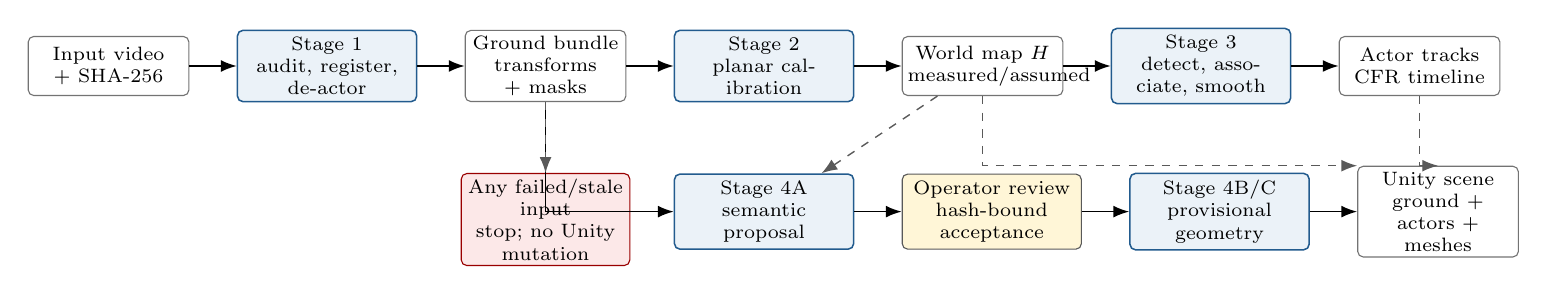
\begin{tikzpicture}[
  font=\scriptsize,
  node distance=5mm and 6mm,
  stage/.style={draw=stageblue, line width=.55pt, rounded corners=2pt, fill=stagefill,
                minimum height=8.5mm, text width=21mm, align=center, inner sep=2.5pt},
  artifact/.style={draw=black!55, rounded corners=2pt, fill=white,
                   minimum height=7.5mm, text width=19mm, align=center, inner sep=2pt},
  review/.style={draw=black!65, rounded corners=2pt, fill=reviewfill,
                 minimum height=8.5mm, text width=21mm, align=center, inner sep=2.5pt},
  reject/.style={draw=red!60!black, rounded corners=2pt, fill=rejectfill,
                 minimum height=7mm, text width=20mm, align=center, inner sep=2pt},
  flow/.style={-{Latex[length=2mm]}, line width=.55pt},
  dep/.style={-{Latex[length=2mm]}, line width=.5pt, dashed, draw=black!65}
]
\node[artifact] (video) {Input video\\+ SHA-256};
\node[stage, right=of video] (s1) {Stage 1\\audit, register, de-actor};
\node[artifact, right=of s1] (ground) {Ground bundle\\transforms + masks};
\node[stage, right=of ground] (s2) {Stage 2\\planar calibration};
\node[artifact, right=of s2] (cal) {World map $H$\\measured/assumed};
\node[stage, right=of cal] (s3) {Stage 3\\detect, associate, smooth};
\node[artifact, right=of s3] (tracks) {Actor tracks\\CFR timeline};

\node[stage, below=9mm of s2] (s4a) {Stage 4A\\semantic proposal};
\node[review, right=of s4a] (human) {Operator review\\hash-bound acceptance};
\node[stage, right=of human] (s4bc) {Stage 4B/C\\provisional geometry};
\node[artifact, right=of s4bc] (unity) {Unity scene\\ground + actors + meshes};
\node[reject, below=9mm of ground] (stop) {Any failed/stale input\\stop; no Unity mutation};

\draw[flow] (video) -- (s1);
\draw[flow] (s1) -- (ground);
\draw[flow] (ground) -- (s2);
\draw[flow] (s2) -- (cal);
\draw[flow] (cal) -- (s3);
\draw[flow] (s3) -- (tracks);
\draw[flow] (ground) |- (s4a);
\draw[dep] (cal) -- (s4a);
\draw[flow] (s4a) -- (human);
\draw[flow] (human) -- (s4bc);
\draw[flow] (s4bc) -- (unity);
\draw[dep] (ground.south) -- ++(0,-3mm) -| (stop.north);
\draw[dep] (tracks.south) |- (unity.north);
\draw[dep] (cal.south) |- (unity.north west);
\end{tikzpicture}
}
\caption{Pipeline and trust boundaries. Solid arrows carry required artifacts; dashed arrows denote validation dependencies. A stage publishes a versioned bundle only after its gate passes. Geometry additionally requires operator acceptance bound to the exact semantic hashes.}
\label{fig:architecture}
\end{figure*}

\end{document}
